\section{Understanding \texttt{.yaml} files} \label{app:yaml}
Simulations in AutoPas are configured using parameters specified in a \texttt{.yaml} file, which defines the conditions of the simulation. The key fields relevant to this thesis are:

\begin{verbatim}
container                        : # List of containers to choose from
verlet-rebuild-frequency         : # Frequency of neighbor list rebuilds
verlet-skin-radius               : # Distance within which a particle is 
                                   # stored in the neighbor list
data-layout                      : # Data storage format (AoS or SoA)
traversal                        : # List of traversals to choose from
newton3                          : # Boolean value determining if Newton's 
                                   # third law is enabled
iterations                       : # Number of iterations
\end{verbatim}

All the \texttt{.yaml} files, used for every simulation, are available \href{https://github.com/xhulia028/GraphView}{\texttt{here}}.


% ================== Freq vs Time =====================
\begin{figure}[htbp]
    \centering
    \vspace{-0.5em}
    \begin{subfigure}[b]{\textwidth}
        \centering
        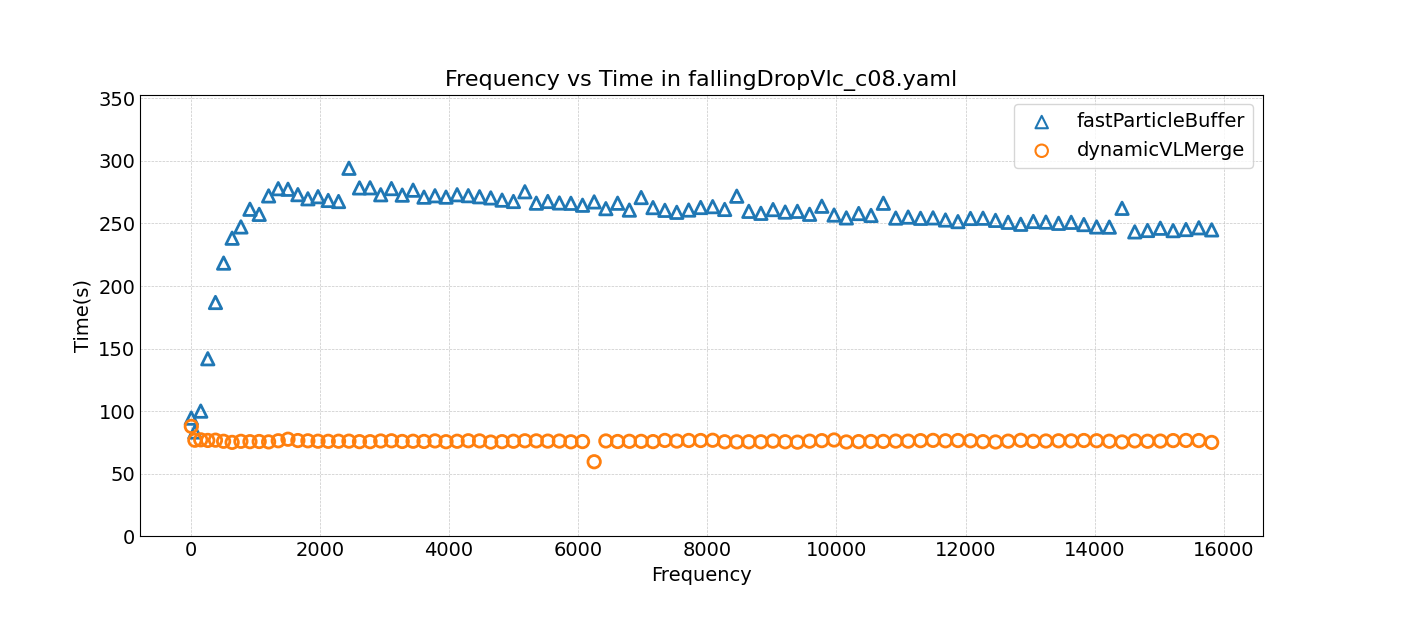
\includegraphics[width=0.9\linewidth]{graphs/fallingDrop/normalExperiments/freq/vlcc08.png}
        \vspace{-0.5em}
        \caption{\scriptsize Falling Drop vlc\_c08}
        \label{fig:vlcc08fallingDrop}
    \end{subfigure}

    \begin{subfigure}[b]{\textwidth}
        \centering
        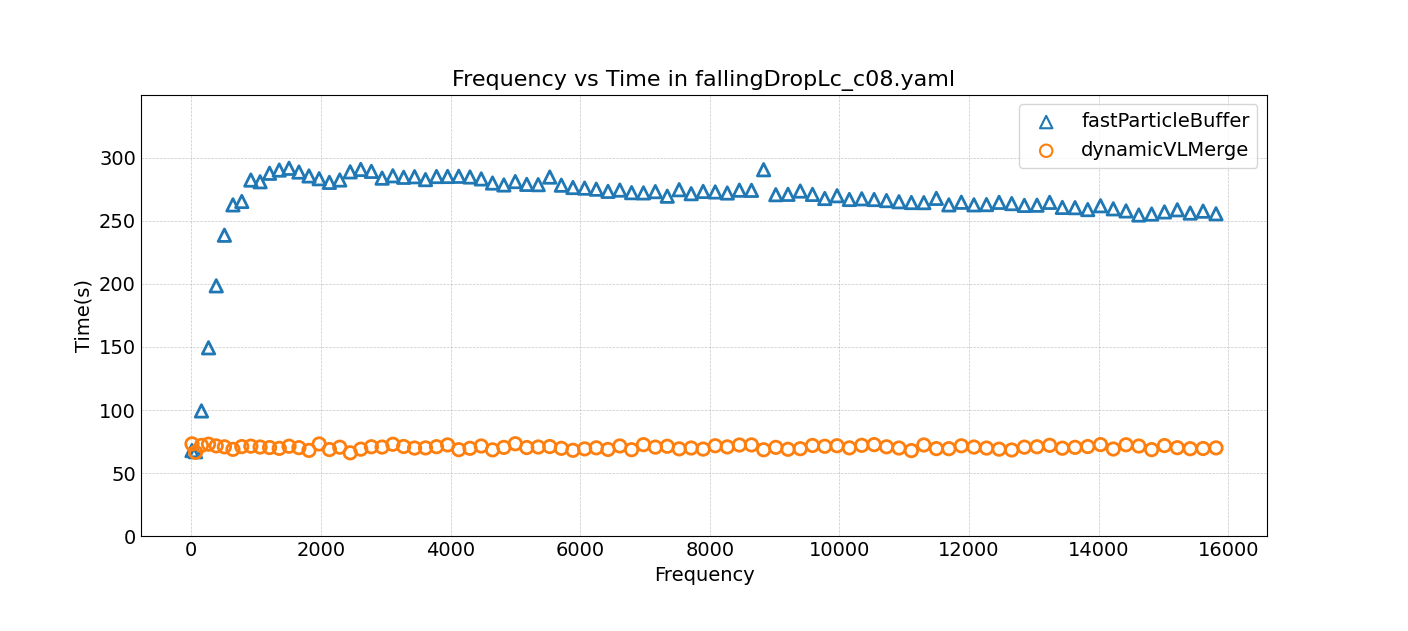
\includegraphics[width=0.9\linewidth]{graphs/fallingDrop/normalExperiments/freq/lcc08.png}
        \vspace{-0.5em}
        \caption{\scriptsize Falling Drop lc\_c08}
        \label{fig:lcc08explodingLiquid}
    \end{subfigure}

    \begin{subfigure}[b]{\textwidth}
        \centering
        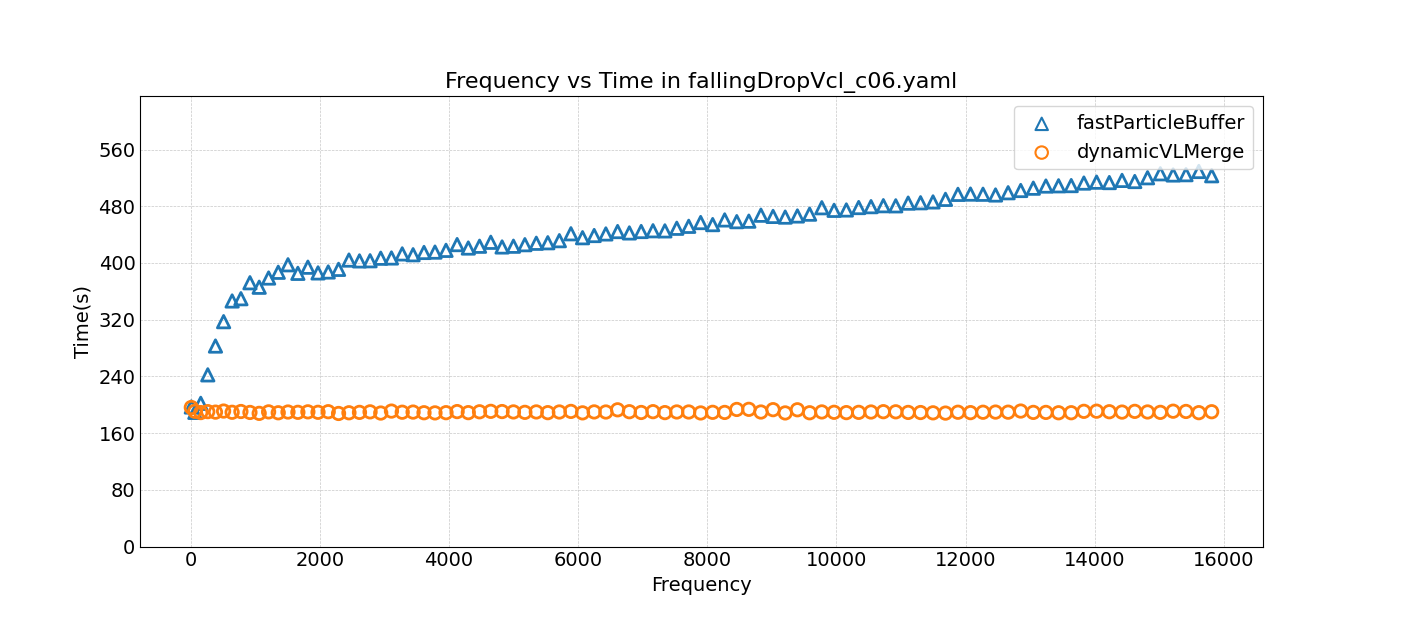
\includegraphics[width=0.9\linewidth]{graphs/fallingDrop/normalExperiments/freq/vclc06.png}
        \vspace{-0.5em}
        \caption{\scriptsize Falling Drop vcl\_c06}
        \label{fig:vclc06constantVelocityCube}
    \end{subfigure}

    \vspace{1em}
    \caption{Comparison of Frequency vs Time for Falling Drop Experiments}
    \label{fig:mainFallingDrop}
\end{figure}


\begin{figure}[htbp]
    \centering
    \vspace{-0.5em}
    \begin{subfigure}[b]{\textwidth}
        \centering
        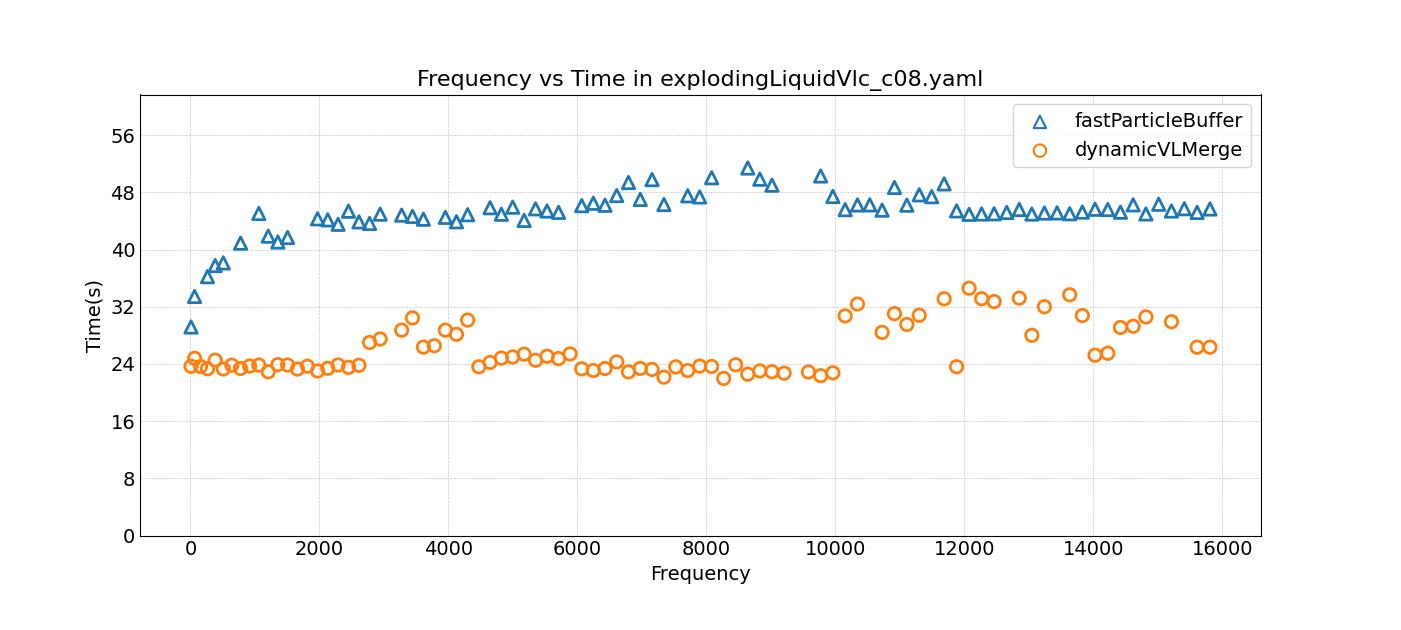
\includegraphics[width=0.9\linewidth]{graphs/explodingLiquid/normalExperiments/freq/vlcc08.png}
        \vspace{-0.5em}
        \caption{\scriptsize Exploding Liquid vlc\_c08}
        \label{fig:vlcc08explodingLiquid}
    \end{subfigure}

    \begin{subfigure}[b]{\textwidth}
        \centering
        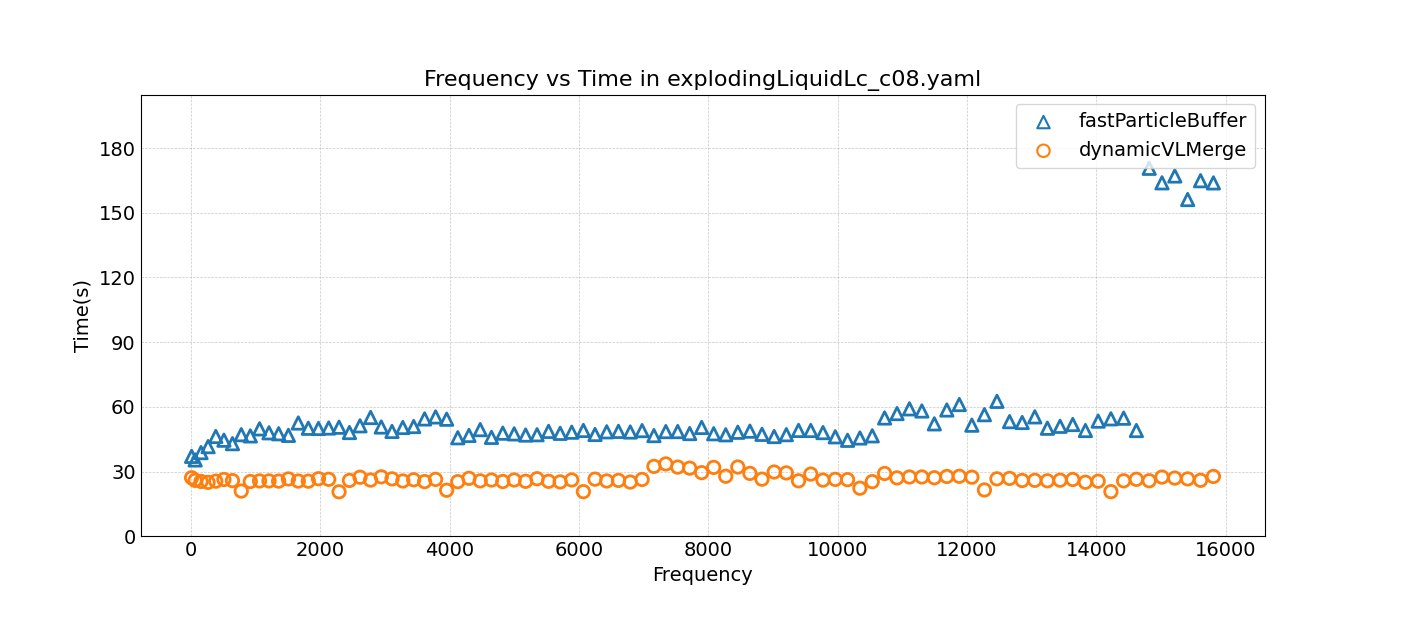
\includegraphics[width=0.9\linewidth]{graphs/explodingLiquid/normalExperiments/freq/lcc08.png}
        \vspace{-0.5em}
        \caption{\scriptsize Exploding Liquid lc\_c08}
        \label{fig:lcc08explodingLiquid}
    \end{subfigure}

    \begin{subfigure}[b]{\textwidth}
        \centering
        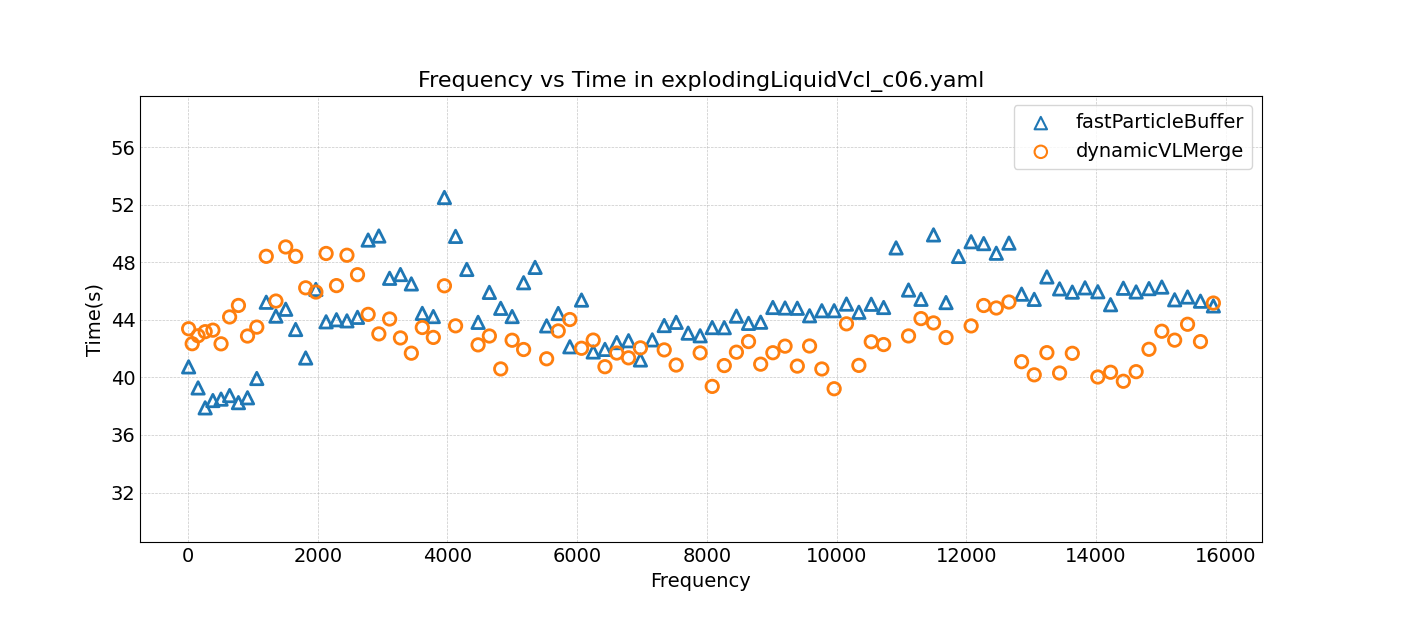
\includegraphics[width=0.9\linewidth]{graphs/explodingLiquid/normalExperiments/freq/vclc06.png}
        \vspace{-0.5em}
        \caption{\scriptsize Exploding Liquid vcl\_c06}
        \label{fig:vclc06explodingLiquid}
    \end{subfigure}

    \vspace{1em}
    \caption{Comparison of Frequency vs Time for Exploding Liquid Experiments}
    \label{fig:mainExplodingLiquid}
\end{figure}


\begin{figure}[htbp]
    \centering
    \vspace{-0.5em}
    \begin{subfigure}[b]{\textwidth}
        \centering
        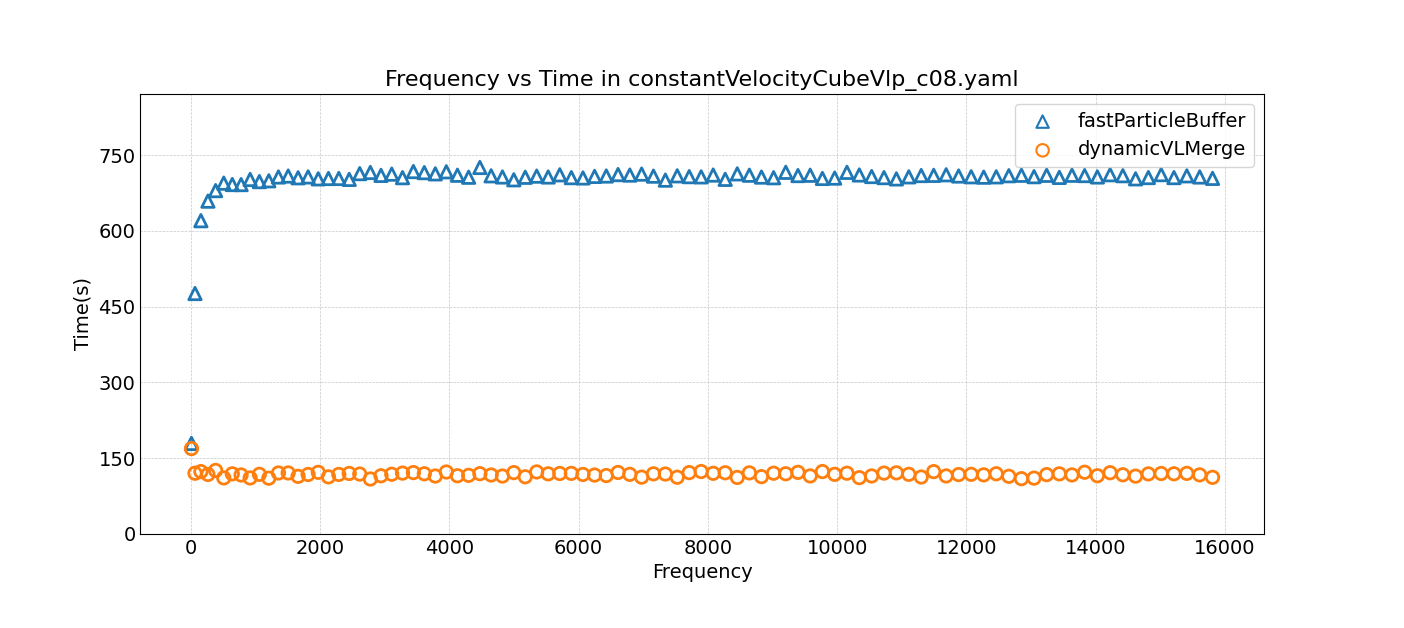
\includegraphics[width=0.9\linewidth]{graphs/constantVelocityCube/normalExperiments/freq/vlpc08.png}
        \vspace{-0.5em}
        \caption{\scriptsize Constant Velocity Cube vlp\_c08}
        \label{fig:vlpc08constantVelocityCube}
    \end{subfigure}

    \begin{subfigure}[b]{\textwidth}
        \centering
        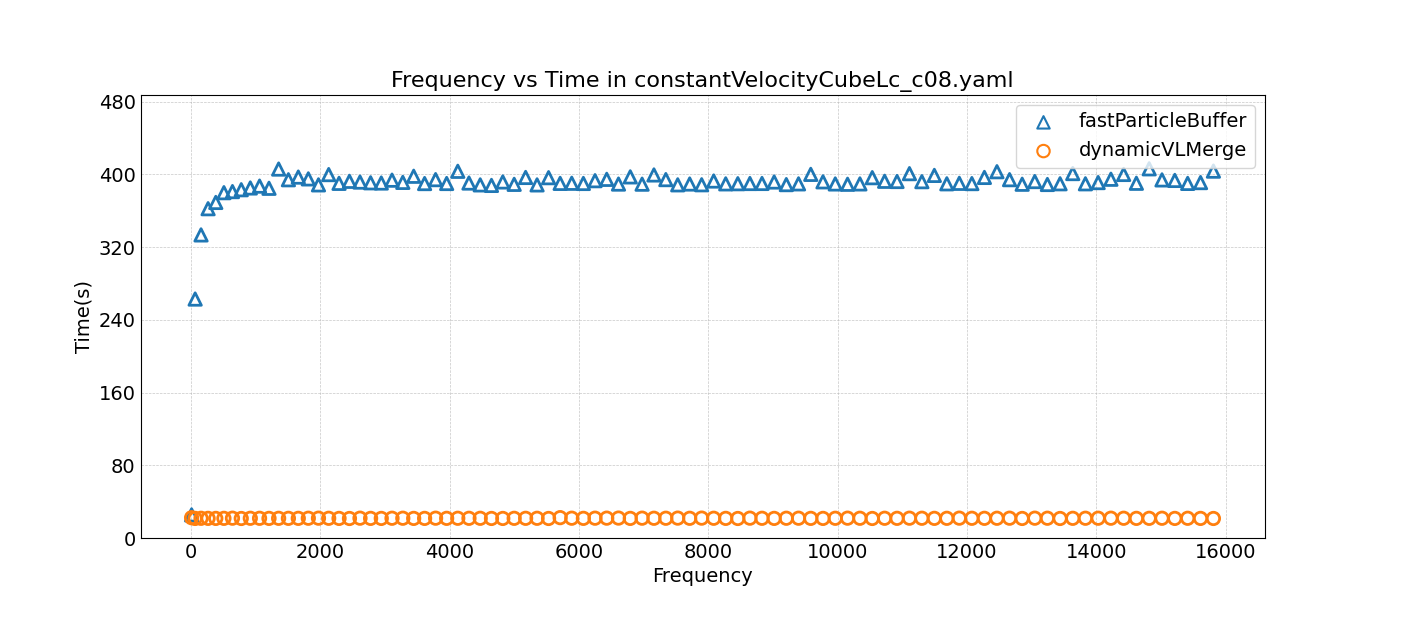
\includegraphics[width=0.9\linewidth]{graphs/constantVelocityCube/normalExperiments/freq/lcc08.png}
        \vspace{-0.5em}
        \caption{\scriptsize Constant Velocity Cube lc\_c08}
        \label{fig:lcc08constantVelocityCube}
    \end{subfigure}

    \begin{subfigure}[b]{\textwidth}
        \centering
        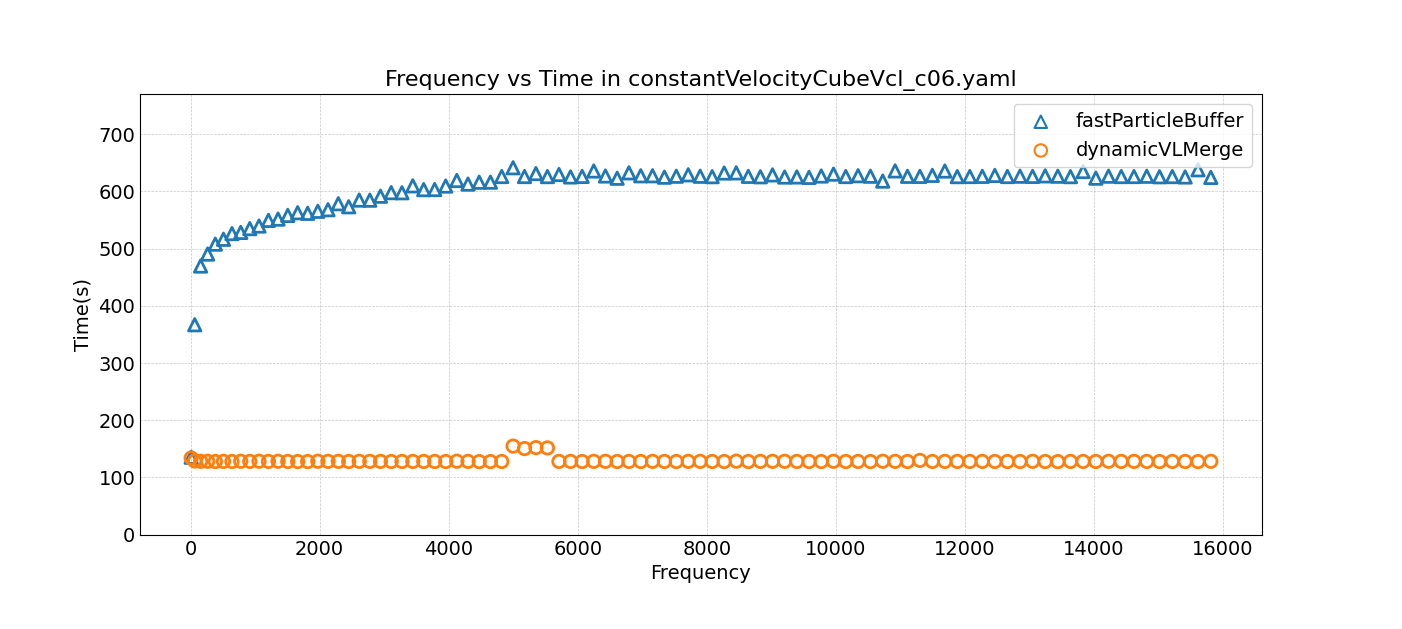
\includegraphics[width=0.9\linewidth]{graphs/constantVelocityCube/normalExperiments/freq/vclc06.png}
        \vspace{-0.5em}
        \caption{\scriptsize Constant Velocity Cube vcl\_c06}
        \label{fig:vclc06constantVelocityCube}
    \end{subfigure}

    \vspace{1em}
    \caption{Comparison of Frequency vs Time for Constant Velocity Cube Experiments}
    \label{fig:mainConstantVelocityCube}
\end{figure}

% ======================================================


% =====================Compute Inter vs Remainder Traversal Exploding Liquid=================================

\begin{figure}[htbp]
    \centering
    \vspace{-0.5em}
    \begin{subfigure}[b]{\textwidth}
        \centering
        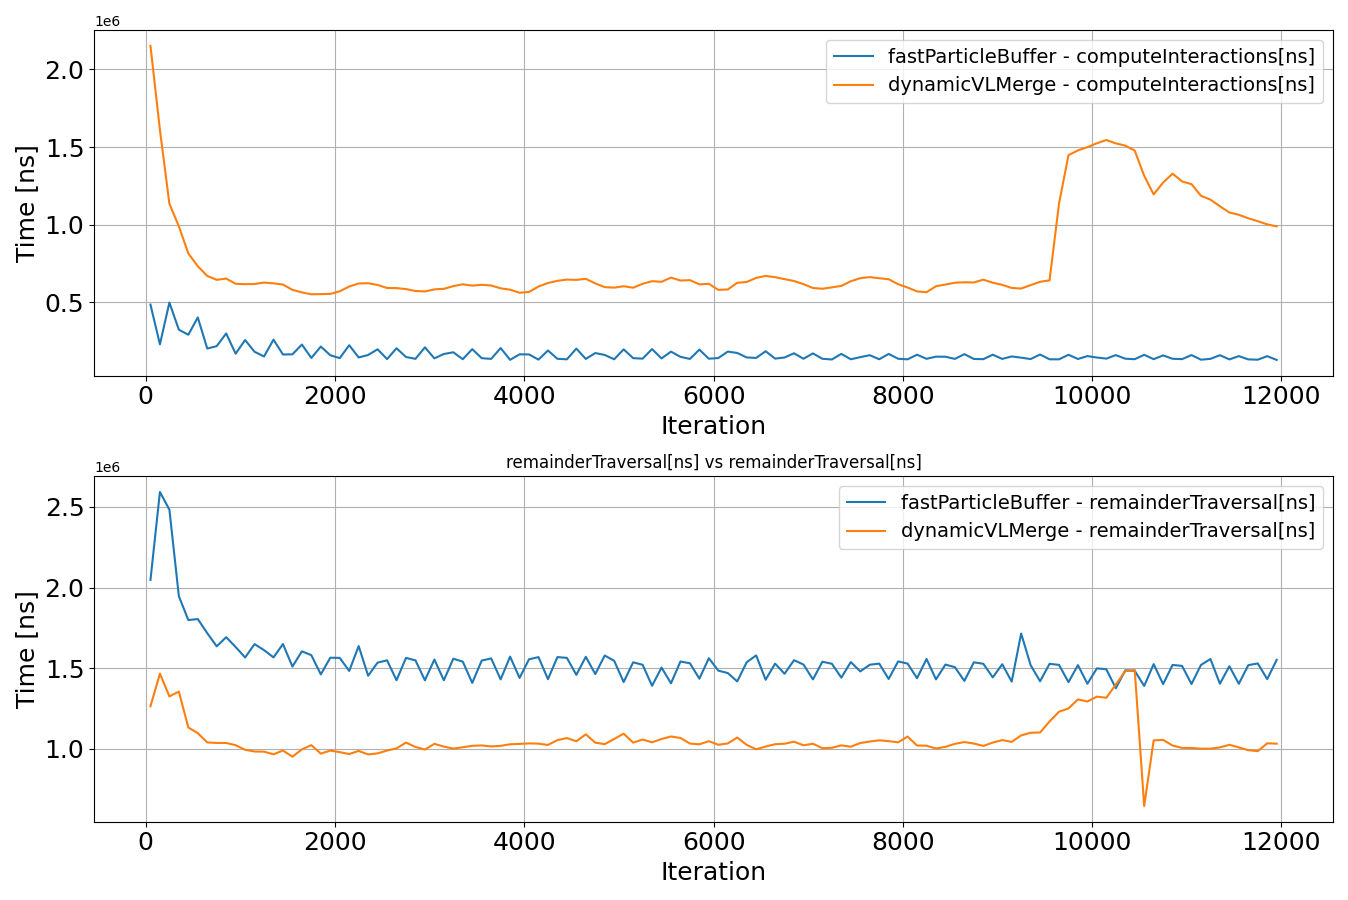
\includegraphics[width=0.9\linewidth]{graphs/explodingLiquid/normalExperiments/freq/vclc0_6inter.png}
        \vspace{-0.5em}
        \caption{\scriptsize Exploding Liquid Vcl\_c06}
        \label{fig:explodingLiquid_vclc0_6inter}
    \end{subfigure}

    \begin{subfigure}[b]{\textwidth}
        \centering
        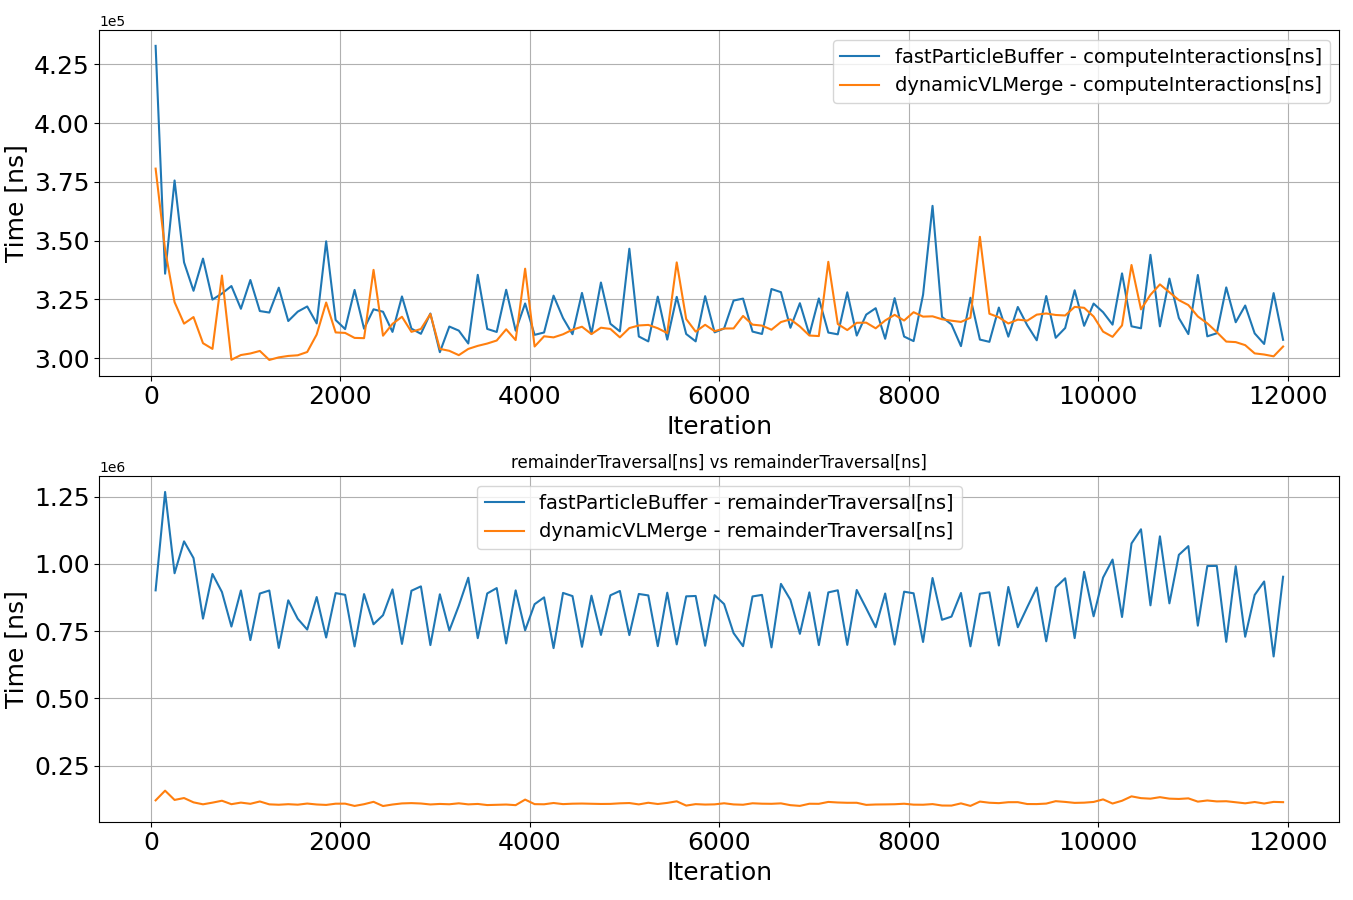
\includegraphics[width=0.9\linewidth]{graphs/explodingLiquid/normalExperiments/freq/vlc_c08inter.png}
        \vspace{-0.5em}
        \caption{\scriptsize Exploding Liquid Vlc\_c08}
        \label{fig:explodingLiquid_vlc_c08inter}
    \end{subfigure}

    \vspace{1em}
    \caption{Comparison of Compute Interactions and Remainder Traversal for Exploding Liquid Experiments}
    \label{fig:mainexplodingLiquid_inter}
\end{figure}
% ======================================================

% ============================== Iteration vs Time ==============================

\begin{figure}[htbp]
    \centering
    \vspace{-0.7em}
    \begin{subfigure}[b]{\textwidth}
        \centering
        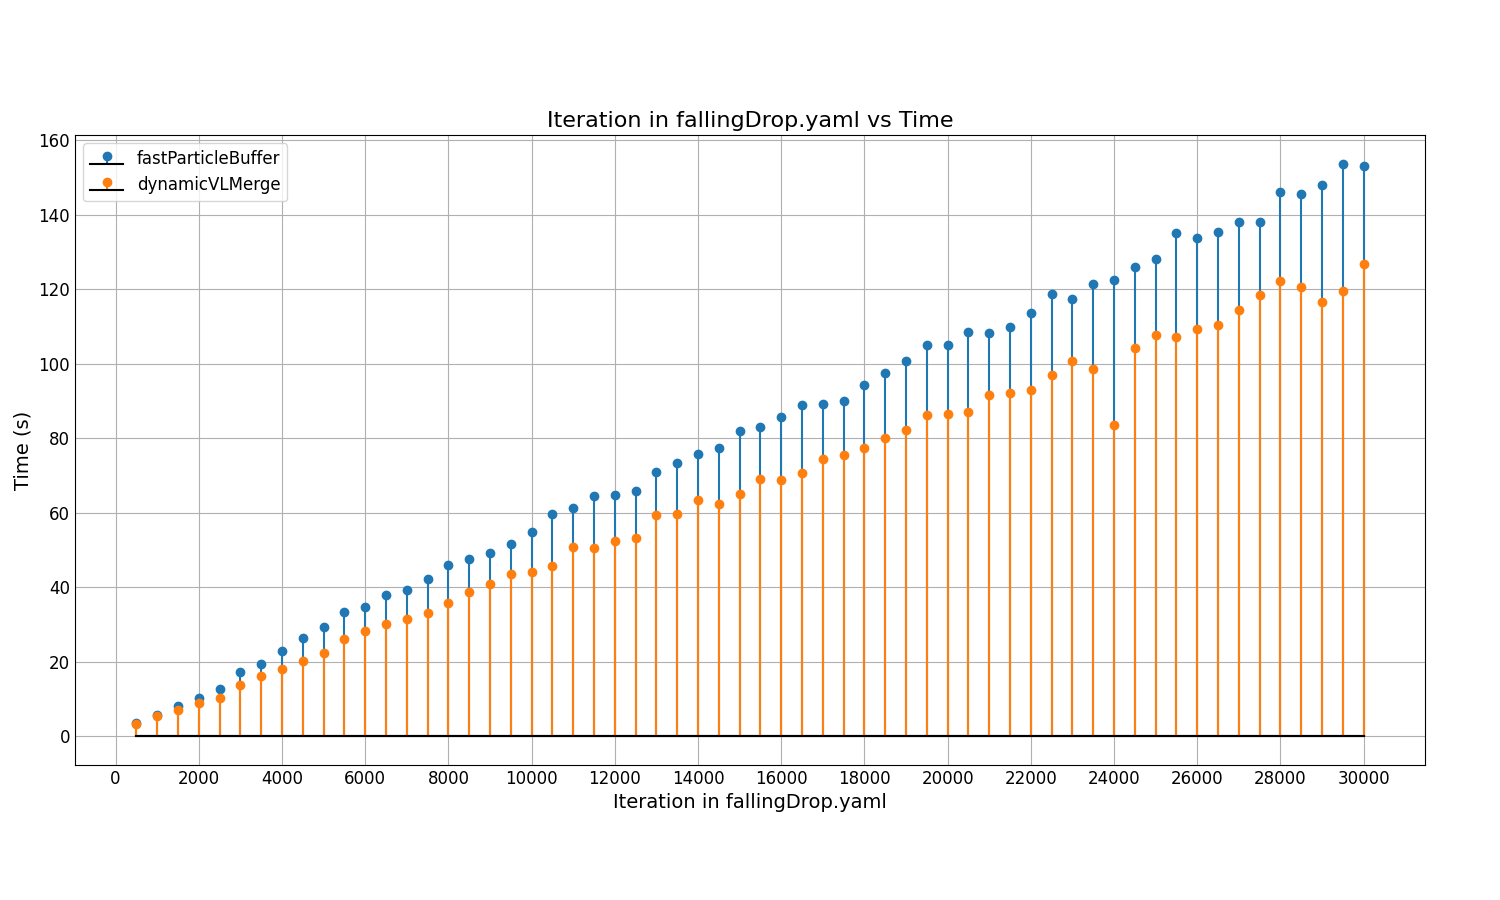
\includegraphics[width=0.85\linewidth]{graphs/fallingDrop/freqvstimeiter.png}
        \vspace{-0.5em}
        \caption{\scriptsize Falling Drop}
        \label{fig:tuningfallingDropIter}
    \end{subfigure}

    \begin{subfigure}[b]{\textwidth}
        \centering
        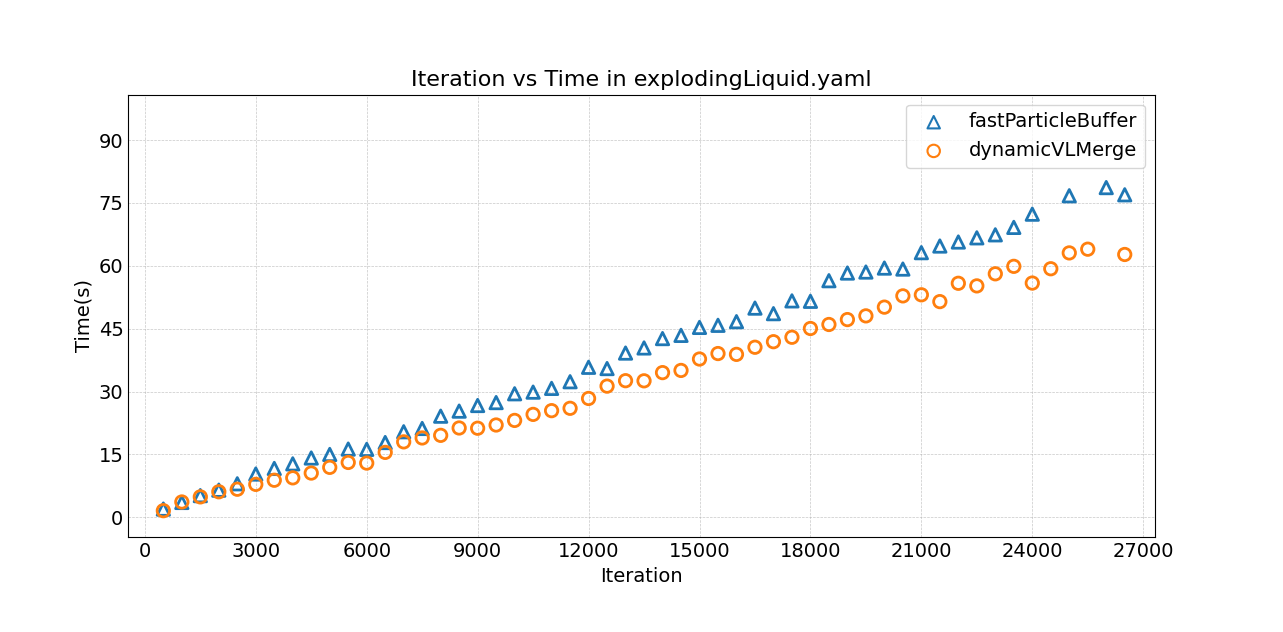
\includegraphics[width=0.85\linewidth]{graphs/explodingLiquid/freqvstimeiter.png}
        \vspace{-0.5em}
        \caption{\scriptsize Exploding Liquid}
        \label{fig:tuningexplodingLiquidIter}
    \end{subfigure}

    \begin{subfigure}[b]{\textwidth}
        \centering
        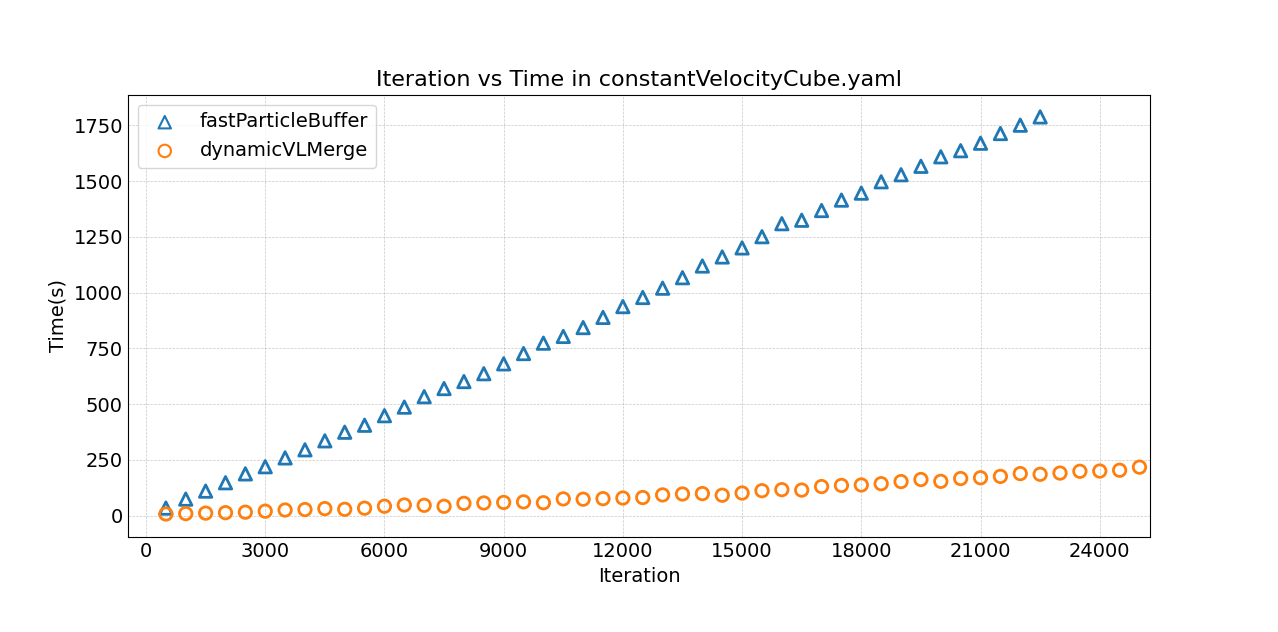
\includegraphics[width=0.85\linewidth]{graphs/constantVelocityCube/freqvstimeiter.png}
        \vspace{-0.5em}
        \caption{\scriptsize Constant Velocity Cube}
        \label{fig:tuningconstantVelocityCubeIter}
    \end{subfigure}

    \vspace{0.5em}
    \caption{Comparison of Frequency vs Iterations with Tuning}
    \label{fig:mainIterWithTuning}
\end{figure}


% ============================== Iteration vs Time Falling Drop ==============================

\begin{figure}[htbp]
    \centering
    \vspace{-0.5em}
    \begin{subfigure}[b]{\textwidth}
        \centering
        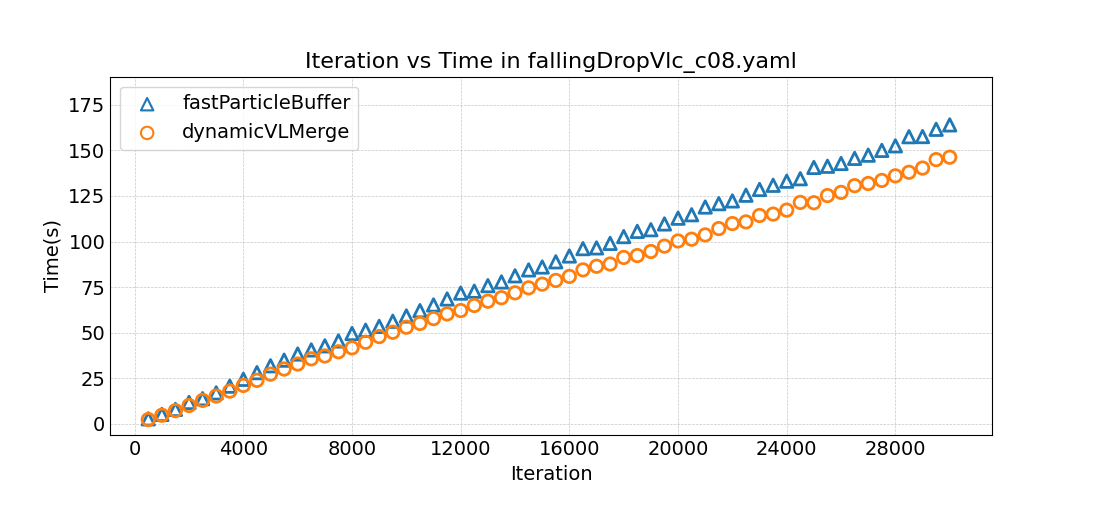
\includegraphics[width=0.9\linewidth]{graphs/fallingDrop/normalExperiments/iter/vlcc08.png}
        \vspace{-0.5em}
        \caption{\scriptsize Falling Drop vlc\_c08}
        \label{fig:vlcc08fallingDropIter}
    \end{subfigure}

    \begin{subfigure}[b]{\textwidth}
        \centering
        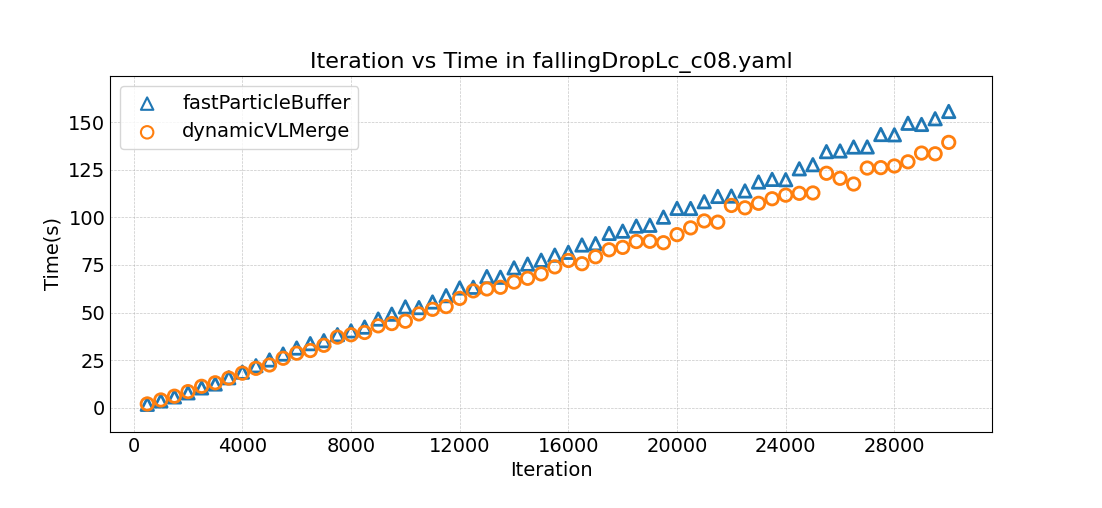
\includegraphics[width=0.9\linewidth]{graphs/fallingDrop/normalExperiments/iter/lcc08.png}
        \vspace{-0.5em}
        \caption{\scriptsize Falling Drop lc\_c08}
        \label{fig:lcc08fallingDropIter}
    \end{subfigure}

    \begin{subfigure}[b]{\textwidth}
        \centering
        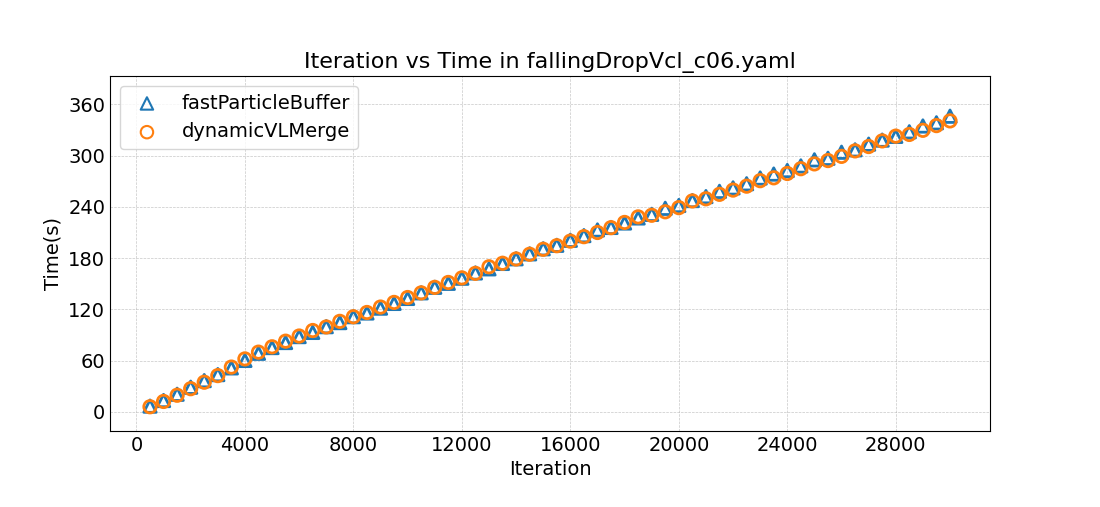
\includegraphics[width=0.9\linewidth]{graphs/fallingDrop/normalExperiments/iter/vclc06.png}
        \vspace{-0.5em}
        \caption{\scriptsize Falling Drop vcl\_c06}
        \label{fig:vclc06fallingDropIter}
    \end{subfigure}

    \vspace{1em}
    \caption{Comparison of Iteration vs Time for Falling Drop Experiments}
    \label{fig:mainfallingDropIter}
\end{figure}


% ============================== Iteration vs Time Exploding Liquid ==============================

\begin{figure}[htbp]
    \centering
    \vspace{-0.5em}
    \begin{subfigure}[b]{\textwidth}
        \centering
        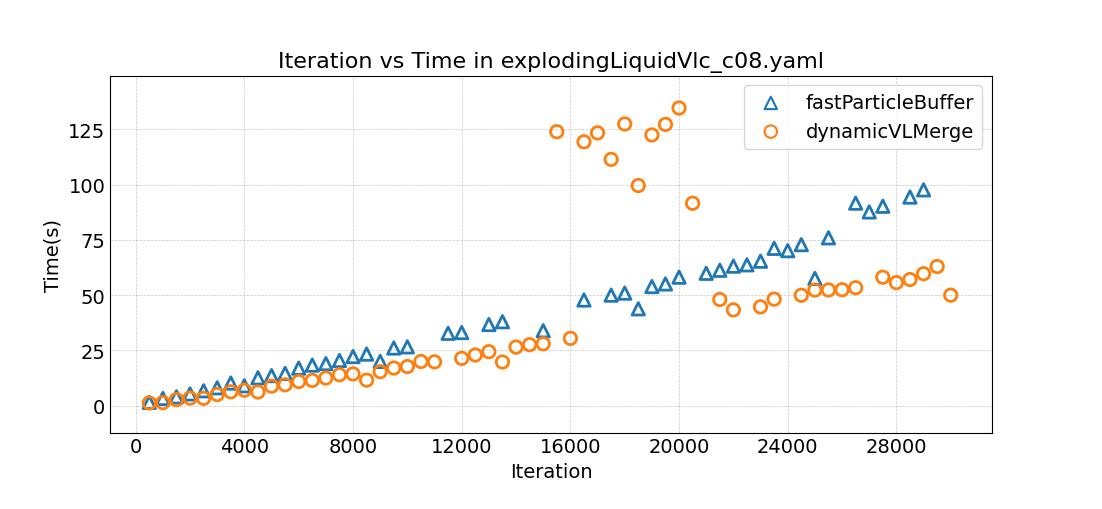
\includegraphics[width=0.9\linewidth]{graphs/explodingLiquid/normalExperiments/iter/vlcc08.png}
        \vspace{-0.5em}
        \caption{\scriptsize Exploding Liquid vlc\_c08}
        \label{fig:vlcc08explodingLiquidIter}
    \end{subfigure}

    \begin{subfigure}[b]{\textwidth}
        \centering
        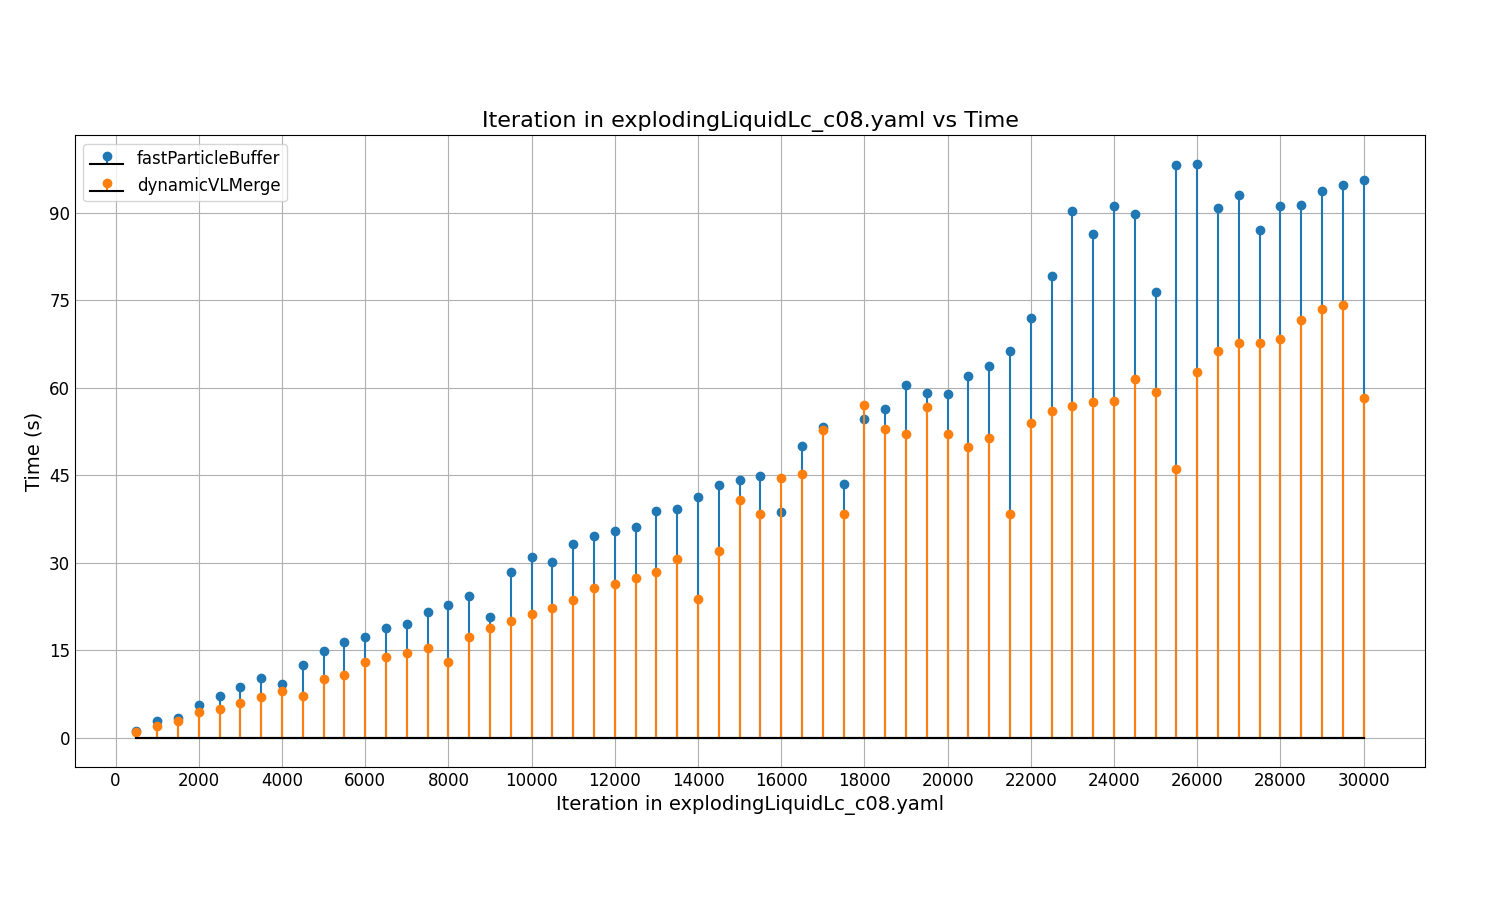
\includegraphics[width=0.9\linewidth]{graphs/explodingLiquid/normalExperiments/iter/lcc08.png}
        \vspace{-0.5em}
        \caption{\scriptsize Exploding Liquid lc\_c08}
        \label{fig:lcc08explodingLiquidIter}
    \end{subfigure}

    \begin{subfigure}[b]{\textwidth}
        \centering
        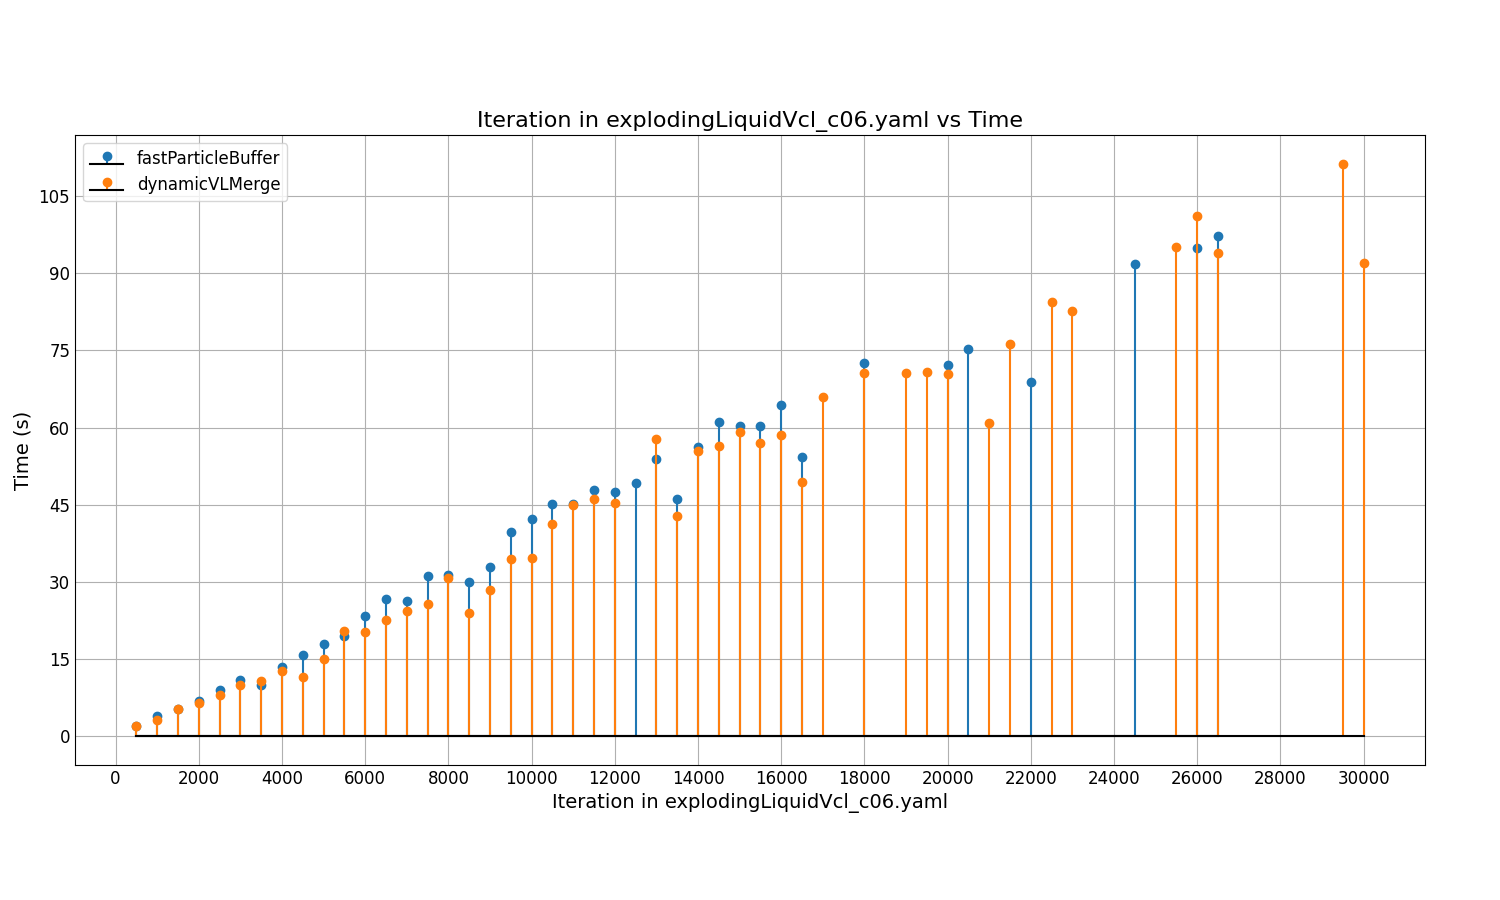
\includegraphics[width=0.9\linewidth]{graphs/explodingLiquid/normalExperiments/iter/vclc06.png}
        \vspace{-0.5em}
        \caption{\scriptsize Exploding Liquid vcl\_c06}
        \label{fig:vclc06explodingLiquidIter}
    \end{subfigure}

    \vspace{1em}
    \caption{Comparison of Iteration vs Time for Exploding Liquid Experiments}
    \label{fig:mainexplodingLiquidIter}
\end{figure}


% ============================== Iteration vs Time Constant velocity cube ==============================

\begin{figure}[htbp]
    \centering
    \vspace{-0.5em}
    \begin{subfigure}[b]{\textwidth}
        \centering
        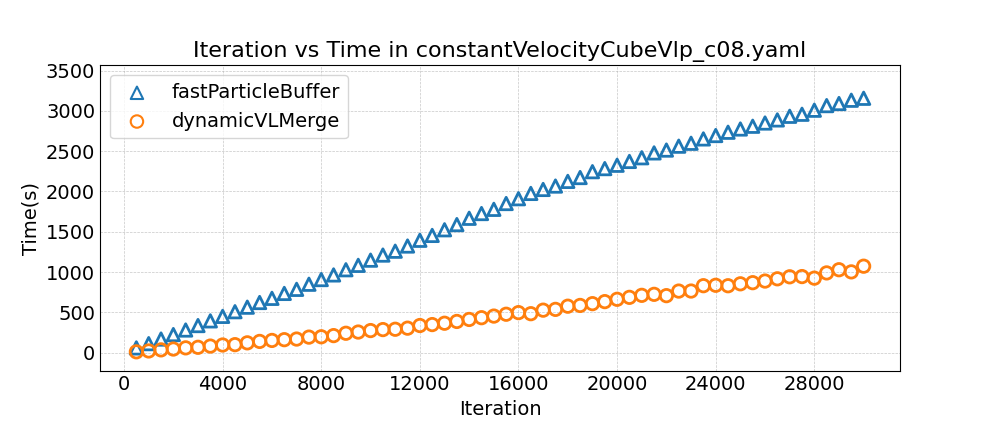
\includegraphics[width=0.9\linewidth]{graphs/constantVelocityCube/normalExperiments/iter/vlpc08.png}
        \vspace{-0.5em}
        \caption{\scriptsize Constant Velocity Cube vlp\_c08}
        \label{fig:vlpc08constantCubeIter}
    \end{subfigure}

    \begin{subfigure}[b]{\textwidth}
        \centering
        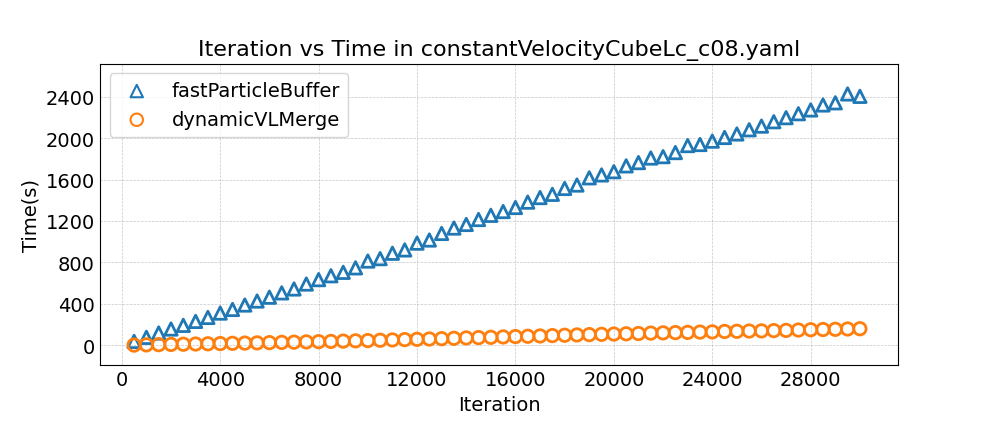
\includegraphics[width=0.9\linewidth]{graphs/constantVelocityCube/normalExperiments/iter/lcc08.png}
        \vspace{-0.5em}
        \caption{\scriptsize Constant Velocity Cube lc\_c08}
        \label{fig:lcc08constantCubeIter}
    \end{subfigure}

    \begin{subfigure}[b]{\textwidth}
        \centering
        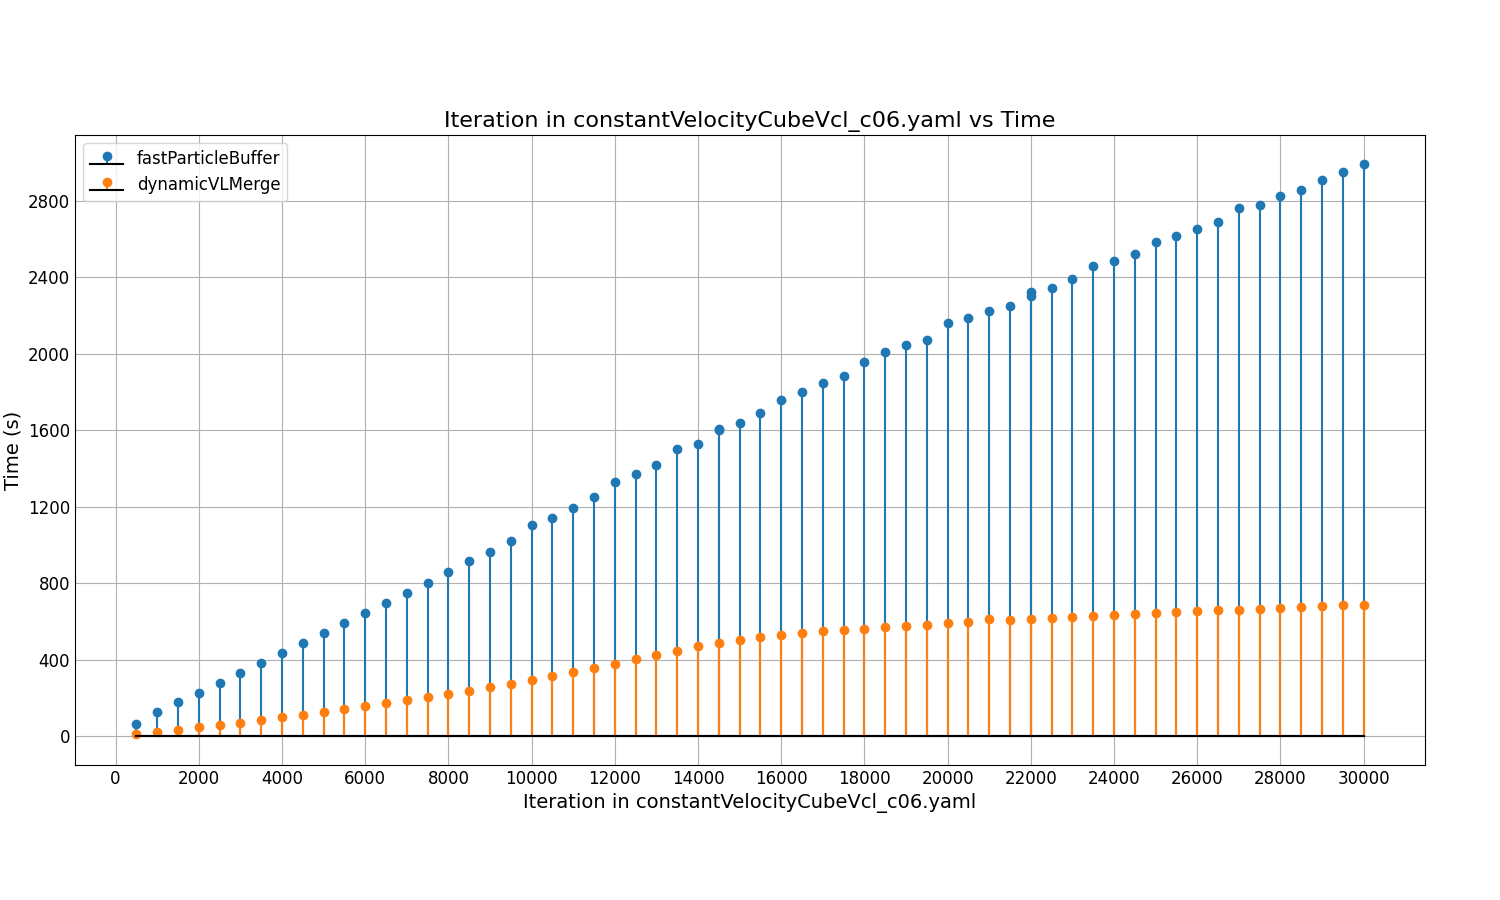
\includegraphics[width=0.9\linewidth]{graphs/constantVelocityCube/normalExperiments/iter/vclc06.png}
        \vspace{-0.5em}
        \caption{\scriptsize Constant Velocity Cube vcl\_c06}
        \label{fig:vclc06constantCubeIter}
    \end{subfigure}

    \vspace{1em}
    \caption{Comparison of Iteration vs Time for Constant Velocity Cube Experiments}
    \label{fig:mainConstantCubeIter}
\end{figure}





% ======================================================



